\documentclass[journal]{IEEEtran}
\usepackage[T1]{fontenc}
\usepackage[utf8]{inputenc}
\usepackage{cite}
\usepackage{amsmath}
\usepackage{graphicx}
\usepackage{booktabs}
\usepackage{url}
\usepackage{hyperref}
\hypersetup{colorlinks=true, urlcolor=blue, citecolor=blue, linkcolor=blue}

\begin{document}

\title{Predicting Missed Outpatient Appointments for Booking under Scarce Clinic Capacity}

\author{Sammy~Niyonkuru}

\markboth{Machine Learning Summative Project}{Niyonkuru: Predicting Missed Outpatient Appointments}

\maketitle

\begin{center}
\noindent
\textbf{GitHub repository:} \url{https://github.com/REPLACE_WITH_YOUR_USERNAME/clinic-appointment-noshow}\\[0.3em]
\textbf{Google Drive folder (anyone with the link):} \url{https://drive.google.com/REPLACE_WITH_SHARE_LINK}\\[0.3em]
\textbf{Video recording (5--10 minutes, camera on):} \url{https://REPLACE_WITH_VIDEO_LINK}
\end{center}

\vspace{0.6em}
\noindent\textit{Replace the three links above before submission. The Drive folder must contain the zipped raw file and the saved models. The video must show your face. See the repository README.}

\begin{abstract}
Missed outpatient appointments waste scarce clinician time, and filling those slots by guesswork crowds the waiting room. This project frames non-attendance as a binary classification task that a booking desk could run before it sends a reminder or double-books a slot. The table is the public Vit\'oria appointment extract released by Hoppen: 110{,}527 visits, of which 110{,}516 remain after removing six impossible ages and five negative booking gaps. About 20.2\% of visits are no-shows. Patients are kept entirely inside one split so that personal history cannot leak a test label into training. Sixteen experiments compare a majority rule and a lead-time rule with logistic regression, random forests, gradient boosting, linear and kernel support-vector machines, and three Keras networks trained through \texttt{tf.data}. On a held-out patient group the best traditional model, an unweighted histogram gradient booster, reaches a test ROC-AUC of 0.748 and a precision--recall AUC of 0.411. The best network, a neighbourhood embedding model, reaches 0.743 and 0.404. Lead time accounts for most of the lift over chance. A threshold that maximises F1 flags many attenders, which is tolerable for a cheap reminder and unacceptable for overbooking. Only a thin high-score tail is precise enough to double-book. The coefficients are not a policy for African clinics: the file is one Brazilian city over six weeks, and published African no-show rates are substantially higher.
\end{abstract}

\begin{IEEEkeywords}
appointment non-attendance, clinic booking, class imbalance, gradient boosting, multilayer perceptron
\end{IEEEkeywords}

\section{Introduction}
The practical problem behind this project is a booking desk with too few clinicians and too many people in the corridor. My aim is to improve delivery in African medical institutions by digitizing how appointments are booked and managed, so that overcrowding and idle slots both shrink. Those two failures are linked. A patient who does not attend leaves a clinician waiting. A clinic that answers by booking extra patients into every slot, without knowing who will come, fills the waiting room and lengthens the queue for people who did attend. Oche and Adamu documented that pattern in the general outpatient department of a teaching hospital in Sokoto: most patients waited between 90 and 180 minutes, and the dominant explanation was a large patient load against a small staff \cite{oche2013}. A classifier does not hire nurses. It can, if it is honest about its errors, tell the desk which booked visits are likely to be empty and which reminders are worth a scarce SMS credit.

Non-attendance is common and uneven. Across 105 studies the average rate is near 23\%, and near 43\% in the African studies, against about 13\% in Oceania \cite{dantas2018}. Long lead time, prior misses, younger adult age, and distance recur as predictors. In the prediction literature, logistic regression still dominates, almost no study beats the attendance base rate on accuracy, and an AUC above 0.9 is exceptional \cite{carreras2020}. A model that always says ``will attend'' looks strong and catches nobody.

This study asks whether a visit-level record that a digital booking system would actually store---who the patient is, when they booked, whether a message was sent, and whether they came last time---can rank upcoming visits by the chance of a no-show well enough to support two different actions. The first action is a reminder, where a false alarm is a message sent to someone who would have come anyway. The second is overbooking, where a false alarm puts two patients in one slot and works directly against the goal of a shorter wait \cite{huang2014}. The same score can serve both actions only if the threshold changes. Treating ``the model'' as a single accuracy number hides that choice.

Facility-level African appointment microdata at this scale are not sitting in open repositories; national electronic-record warehouses are not public extracts. I therefore use the public extract of appointments from Vit\'oria, Esp\'irito Santo, Brazil, published by Hoppen \cite{hoppen2016}. It clears the size rule, it has a categorical label, and it is administrative rather than a toy generator. It is also the wrong country. I treat that as a limit on what may be claimed, not as a detail to bury in the last paragraph. Lead time and prior non-attendance travel better across health systems than a neighbourhood code learned in one Brazilian city \cite{dantas2018,mohammadi2018}. The numerical thresholds in this paper should not be copied into a clinic that has not logged its own outcomes.

\section{Literature Review}
\subsection{What drives a missed visit}
Dantas \emph{et al.} find high lead time and prior no-show history to be the determinants most often significant, with younger adults, lower socioeconomic status, distance, and public coverage appearing often \cite{dantas2018}. Their African mean, 43\%, is about twice the Vit\'oria rate, so a probability fit here will be the wrong prior for many of the clinics this mission cares about, even if the direction of the lead-time effect travels.

The reminder evidence does not agree with itself, and the disagreement is the point. Kheirkhah \emph{et al.} estimated an 18.8\% no-show rate in Veterans Health Administration clinics and a cost of \$196 per miss in 2008; a centralised telephone reminder moved one group only from 16.3\% to 15.8\% \cite{kheirkhah2016}. Thomas, Lawani, and James, in a trial at a psychiatric hospital in Benin City, found that SMS reminders nearly doubled attendance and cut the adjusted risk of a missed next visit by about half \cite{thomas2017}. That trial is one diagnosis and not a general outpatient department. Akhigbe and colleagues had already shown missed first appointments to be common in a Nigerian psychiatric clinic \cite{akhigbe2014}. A blanket reminder in a system that already attends most visits is a different intervention from a message where non-attendance is the norm. This project therefore separates ``who should receive a scarce reminder'' from ``message every booking.''

Mohammadi \emph{et al.} studied community health centres, closer to a scarce-resource setting than a tertiary hospital \cite{mohammadi2018}. Lead time, prior misses, phone ownership, tobacco use, and days since the last visit dominated 73{,}811 appointments, and a naive Bayes model was reported near an AUC of 0.86. This extract has no phone flag, no tobacco field, and no reason for the visit, so I should not expect that number. Carreras-Garc\'ia \emph{et al.} already warn that accuracy above the show rate is rare and that an AUC above 0.9 is an outlier \cite{carreras2020}. Huang and Hanauer showed that individual no-show probabilities can beat flat overbooking in a U.S. paediatric simulation \cite{huang2014}. Their costs are not the costs of a Sokoto waiting room \cite{oche2013}. I report a high-precision operating point and a reminder operating point separately, and I label the weights as scenarios.

\subsection{Reminders, access, and what a classifier is for}
A Cochrane review found that mobile-phone message reminders improve attendance relative to no reminder \cite{gurol2013}. That supports putting a message in the booking system. It does not say every booking should get one, and it does not make a Brazilian SMS coefficient causal. In this file, messages were not sent for same-day visits, so a crude SMS comparison is mixed up with lead time. Levesque, Harris, and Russell treat access as the ability to perceive, reach, pay for, and engage with care, not merely the existence of a clinic \cite{levesque2013}. A long lead time is a slot the clinic offered. Calling the resulting no-show a patient failure points the intervention at the wrong place. Holst and colleagues, and the WHO digital-health strategy, make the system-level version of that argument: tools that ignore language, connectivity, and co-design do not strengthen a health system \cite{holst2020,who2021}. Ranking Vit\'oria visits tests whether the stored fields separate the label. It is not a deployment.

\subsection{Learning methods and their failure modes}
Logistic regression is the default in this literature because a few monotone variables often carry the signal and the coefficients can be read \cite{carreras2020}. It is high-bias when the log-odds are not linear \cite{hastie2009,geman1992}. Forests reduce that bias and overfit if leaves are pure \cite{breiman2001}. Boosting keeps the trees small and shrinks each update \cite{friedman2001}. A linear SVM should land near logistic regression; a radial-basis kernel can bend the boundary and does not scale comfortably to 10\textsuperscript{5} rows, so I fit it on a subsample on purpose \cite{cortes1995}. A network can embed a neighbourhood instead of using a hand-built rate \cite{goodfellow2016}, and dropout, batch normalisation, and Adam are the usual controls \cite{srivastava2014,ioffe2015,kingma2015}. None of that promises a gain over boosting if the label is mostly lead time. A loss to the booster is an allowed result.

Two metrics are easy to misuse. ROC-AUC can look fine while precision stays poor under a 20\% positive class; the precision--recall curve is the stricter picture \cite{saito2015}. Accuracy at 0.5 is not comparable across reweighted models. Class weights, and synthetic oversampling such as SMOTE \cite{chawla2002}, change what the score means. I use weights in some runs only, and I do not invent minority rows. Kaufman \emph{et al.} describe how labels leak into features \cite{kaufman2012}. The leak I am guarding against is a row-wise split plus a prior no-show rate computed on the whole file, which would let a training visit see a test visit's outcome. Rajkomar and colleagues note that an acceptable average AUC can still concentrate errors on a group the clinic should not ignore \cite{rajkomar2018}. Age is the slice I check.

\section{Methodology}
\subsection{Data and label}
The source file is the May 2016 public release of 110{,}527 appointment rows \cite{hoppen2016}. It is not a scikit-learn or Keras example set, and it was not simulated for this project. Each row is one appointment. The columns are a patient identifier, an appointment identifier, sex, the booking timestamp, the appointment date, age, neighbourhood, a scholarship flag for Bolsa Familia, hypertension, diabetes, alcoholism, a handicap code, whether an SMS was received, and \texttt{No-show}. In this file, \texttt{No-show = Yes} means the patient did not attend. That polarity is the opposite of ordinary English and is the label used throughout: the positive class is a missed visit. The source spells hypertension and handicap incorrectly; the text uses the ordinary spellings and the pipeline keeps stable feature names.

Booking timestamps are UTC. Appointment dates are stored at UTC midnight as date labels, not instants. Lead time is the calendar-day gap between that date and the booking shifted to UTC$-3$. A raw timestamp difference would mark same-day afternoon bookings as negative waits. Five rows still had a negative lead and were dropped, as were six ages outside 0--110. No appointment identifier was duplicated. The cleaned table has 110{,}516 visits from 62{,}296 patients, 22{,}311 of them no-shows (20.19\%). Appointment dates run from 29 April to 8 June 2016; bookings go back to 10 November 2015. There are 81 neighbourhoods. About 65\% of visits are by women and 9.8\% carry the scholarship flag. The handicap field is an integer from 0 to 4, not a binary flag.

\subsection{Features}
The features were added in three blocks so that later experiments can show what each block is worth.

The demographic and clinical block is age, sex, scholarship, hypertension, diabetes, alcoholism, and the handicap level. These are known at booking and are the covariates a clerk already types. On their own they should be weak, because Dantas \emph{et al.} do not list diagnosis flags as the dominant attendance predictors \cite{dantas2018}.

The scheduling block adds lead time in days, the logarithm of one plus lead time, a same-day indicator, the local hour of the booking, weekday dummies with Monday as the reference, and the SMS flag. Same-day is kept because the association is a cliff, which a linear model cannot make out of a straight lead-time term. The three lead-time columns will share credit, so a single coefficient on raw days is not interpretable alone. SMS was never sent for same-day visits and was sent for about half of later visits, so a crude SMS effect is confounded with lead time. The results check the rate inside lead-time bins before any coefficient is discussed.

The history block is computed inside each patient, after sorting by appointment date, booking time, and appointment identifier. Prior visit count, prior no-show count, and the gap in days since the previous appointment use only earlier rows. The current label is subtracted from the running sum, which the unit tests check. First visits, which have no personal history, receive the training base rate as a placeholder for the prior rate and the training median gap for the day count, plus an indicator that the visit is the first in the extract. Using zero as the prior rate would have described every new patient as a perfect attender.

Neighbourhood is not one-hot encoded. Two training-only summaries are used instead. Frequency is the share of training visits in that neighbourhood. The target code is a smoothed no-show mean, $(s + 30\bar{y})/(n+30)$, with out-of-fold means inside the training split. The folds are grouped by patient, so a patient's own visits do not form the code applied to those same visits \cite{kaufman2012}. Validation and test neighbourhoods that never appear in training fall back to the training base rate. Unseen levels are not dropped, because a new neighbourhood is a real booking event. A third representation, used only by the last neural net, replaces both hand-built codes with an integer id and a learned embedding. The id map is fit on training neighbourhoods; unseen names become index 0.

\subsection{Split, metrics, and thresholds}
Patients, not rows, are assigned to splits. A stratified shuffle on three patient-level strata---never missed, missed fewer than half of their visits, missed at least half---holds out 15\% of patients for test and then 15\% of all patients for validation. The resulting visit counts are 77{,}054, 16{,}736, and 16{,}726. No-show rates are 20.19\%, 20.25\%, and 20.10\%. The visit shares are not exactly 70/15/15 because patients contribute different numbers of rows; the patient shares are. History for a test patient uses only that patient's earlier test visits. Those labels never enter training. They would be known to a clinic on the morning of a later visit, so using them at evaluation is the deployment rule, not a leak.

Hyperparameters and decision thresholds are chosen on validation scores only. The test set is scored after that lock. The threshold-free metrics are ROC-AUC and average precision (the area under the precision--recall curve). At a chosen threshold I report precision, recall, F1, specificity, and accuracy, plus a confusion matrix for the two selected models. Accuracy is reported so that the majority baseline is visible. It is not the selection metric. The default operating point maximises validation F1. Three other policies are locked on validation and then applied once to the test scores of the best probability model: a reminder scenario with relative costs 1 for a false positive and 3 for a false negative; an overbooking scenario with costs 5 and 1, because an extra person in the room is the harm this mission is trying to avoid; and a capacity rule that flags the top 20\% of scores, as if airtime or staff time covered only one booking in five. The cost weights are illustrations. They are not prices from Vit\'oria or from any African facility.

Brier score is reported for models that output probabilities. A reweighted model can rank well and still be a bad probability. Overbooking needs the second property more than the first \cite{huang2014}.

\subsection{Experiments}
Table~\ref{tab:experiments} lists sixteen runs. The seed is 42. E0 always predicts attendance. E1 scores lead time and takes the day cutoff that maximises validation F1. E2--E5 are L2 logistic regressions, standardised inside the pipeline: demographics only; then scheduling with balanced class weights; then the full set at $C=1$; then $C \in \{0.01,0.1,1,10\}$ chosen by validation ROC-AUC. Collinear lead-time terms are read as a group.

E6 is a forest of 200 trees, depth at most 8, at least 20 visits per leaf, and \texttt{balanced\_subsample} weights \cite{breiman2001}. E7 is the variance probe: 80 trees, unlimited depth, leaves of one, each tree on 45\% of rows \cite{geman1992}. E8 sits between them (250 trees, depth 16, leaf 5). E9 is histogram gradient boosting with learning rate 0.08, depth 6, at most 250 iterations, L2 of 0.1, leaf size 30, class weights, and early stopping on an internal 12\% of training rows \cite{friedman2001}. E10 drops the class weights so calibration can be compared with ranking. E11 is a balanced linear SVM with $C \in \{0.1,1,10\}$ chosen on validation ROC-AUC; its scores are margins. E12 is a radial-basis SVM ($C=1$, $\gamma=\texttt{scale}$) fit on 8{,}000 stratified training rows, because a kernel method on the full table was not a responsible use of this machine \cite{cortes1995}.

E13--E15 are Keras models on \texttt{tf.data} pipelines (batch 512, prefetch). E13 is sequential, widths 64 and 32, ReLU, no dropout, no class weights, Adam at $10^{-3}$ \cite{kingma2015}. E14 adds a 128-unit layer, batch normalisation, dropout 0.3 then 0.2, L2 of $10^{-4}$, weights $n/(2n_c)$, and Adam at $5\times 10^{-4}$ \cite{ioffe2015,srivastava2014}. E15 is a functional model: a numeric tower plus a neighbourhood embedding of dimension 8, with the hand-built location rates withheld. Early stopping restores the weights with the best validation ROC-AUC, computed in scikit-learn each epoch (patience 4 or 5), not Keras's batch-wise AUC. Learning curves use three-fold ROC-AUC for the logistic model and a depth-8 forest of 80 trees. Permutation importance shuffles columns of a 4{,}000-row validation subsample, four times.

Every run is logged with Weights \& Biases in offline mode. The run directories are under \texttt{artifacts/wandb}, and the table that the report uses is \texttt{artifacts/metrics/experiment\_table.csv}. The raw CSV is not in the git repository. A download helper fetches the public file if it is absent.

\begin{table*}[t]
\caption{Held-out comparison. Thresholds maximise validation F1 except for E0, which always predicts attendance. Gap is training ROC-AUC minus validation ROC-AUC. AP is average precision.}
\label{tab:experiments}
\centering
\footnotesize
\begin{tabular}{llcccccccc}
\toprule
ID & Model and the change being tested & Val AUC & Val AP & Test AUC & Test AP & Test F1 & Test recall & Gap \\
\midrule
E0 & Always predict attendance & 0.500 & 0.202 & 0.500 & 0.201 & 0.000 & 0.000 & 0.000 \\
E1 & Score = lead time in days & 0.698 & 0.304 & 0.696 & 0.306 & 0.430 & 0.866 & 0.001 \\
E2 & Logistic, demographics only, $C=1$ & 0.544 & 0.219 & 0.539 & 0.215 & 0.337 & 0.834 & 0.006 \\
E3 & Logistic, add scheduling, balanced & 0.722 & 0.349 & 0.713 & 0.334 & 0.438 & 0.731 & 0.003 \\
E4 & Logistic, add history, $C=1$ & 0.734 & 0.384 & 0.726 & 0.373 & 0.441 & 0.761 & 0.001 \\
E5 & Logistic, $C$ chosen on validation & 0.734 & 0.384 & 0.726 & 0.373 & 0.441 & 0.761 & 0.001 \\
E6 & Forest, depth 8, leaf 20 & 0.747 & 0.416 & 0.743 & 0.401 & 0.454 & 0.744 & 0.019 \\
E7 & Forest, unlimited depth, leaf 1 & 0.749 & 0.410 & 0.737 & 0.389 & 0.445 & 0.762 & 0.250 \\
E8 & Forest, depth 16, leaf 5 & 0.754 & 0.425 & 0.746 & 0.403 & 0.457 & 0.783 & 0.131 \\
E9 & Boosting, class-weighted & 0.757 & 0.432 & 0.748 & 0.410 & 0.452 & 0.693 & 0.013 \\
E10 & Boosting, no class weights & 0.758 & 0.436 & 0.748 & 0.411 & 0.454 & 0.733 & 0.017 \\
E11 & Linear SVM, $C$ chosen on validation & 0.734 & 0.385 & 0.726 & 0.373 & 0.441 & 0.729 & 0.001 \\
E12 & RBF SVM on 8{,}000 training rows & 0.711 & 0.343 & 0.712 & 0.338 & 0.436 & 0.828 & 0.119 \\
E13 & MLP, 64--32, no weights & 0.744 & 0.407 & 0.737 & 0.395 & 0.447 & 0.736 & 0.015 \\
E14 & MLP, dropout, batch norm, weights & 0.746 & 0.409 & 0.739 & 0.398 & 0.451 & 0.773 & 0.009 \\
E15 & MLP, neighbourhood embedding & 0.749 & 0.412 & 0.743 & 0.404 & 0.449 & 0.728 & 0.014 \\
\bottomrule
\end{tabular}
\end{table*}

\section{Results}
\subsection{The label is mostly a booking-gap problem}
On the training patients, same-day visits are 34.8\% of rows and have a no-show rate of 4.5\%. The rate is already 22.6\% one or two days later and 32.3\% at fifteen to thirty days. The step off the same day is larger than every later step. Age moves as the reviews describe \cite{dantas2018}: 24.4\% at ages 18--29 and 15.1\% at 60 and above (Fig.~\ref{fig:lead}, Fig.~\ref{fig:age}). Fig.~\ref{fig:sms} shows the SMS confounder. No messages were sent for waits under three days. From three days on, the SMS group has a lower no-show rate than the no-message group in the same bin (29.3\% versus 36.9\% at fifteen to thirty days).

\begin{figure}[t]
\centering
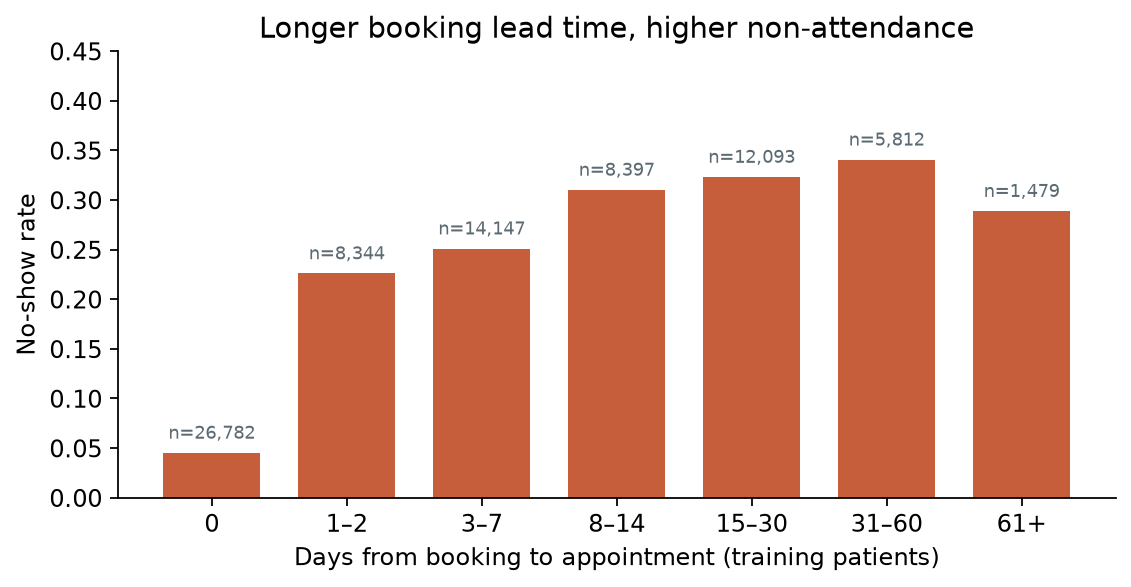
\includegraphics[width=\columnwidth]{../artifacts/figures/noshow_by_lead.png}
\caption{No-show rate by booking lead time on training patients. The same-day bar is the operational fact: offering a near-term slot changes the base rate more than a fine retuning of $C$.}
\label{fig:lead}
\end{figure}

\begin{figure}[t]
\centering
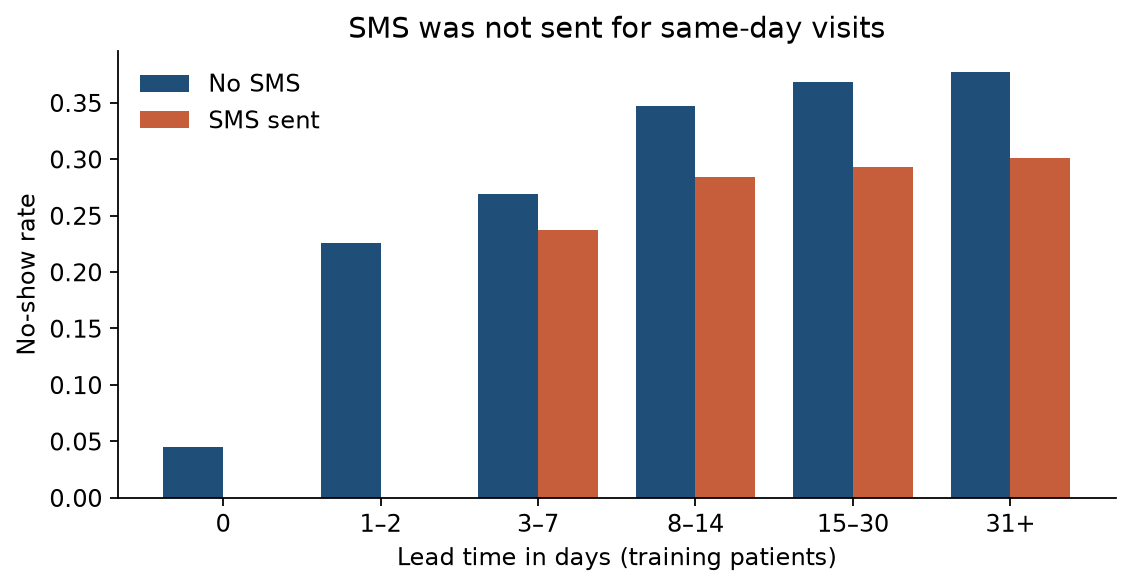
\includegraphics[width=\columnwidth]{../artifacts/figures/sms_by_lead.png}
\caption{SMS was not used for short-notice visits. Inside a lead-time bin, the message is associated with a lower no-show rate, so a crude SMS comparison has the wrong sign.}
\label{fig:sms}
\end{figure}

\begin{figure}[t]
\centering
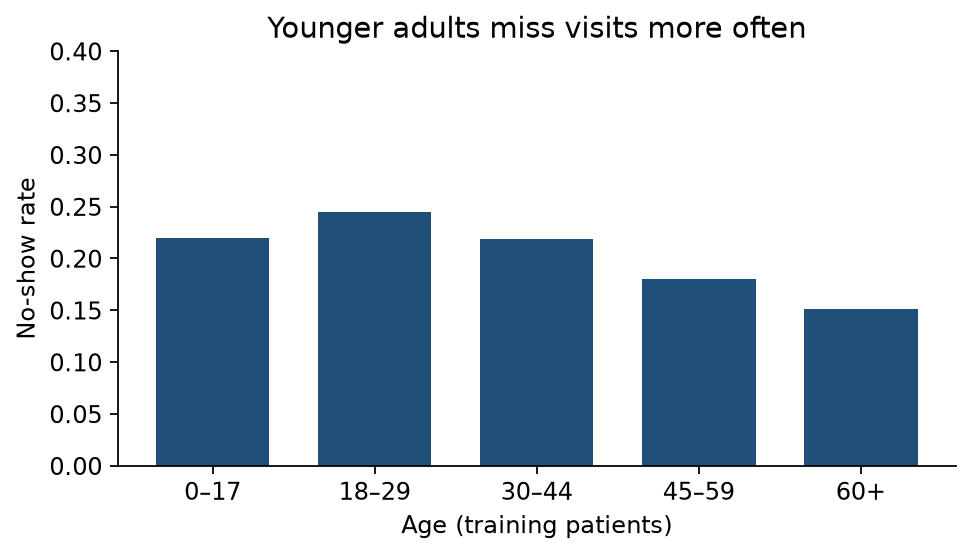
\includegraphics[width=\columnwidth]{../artifacts/figures/noshow_by_age.png}
\caption{Training no-show rate by age. Younger adults miss more often, which matches the determinant reviews and later shows up as unequal recall.}
\label{fig:age}
\end{figure}

E0's test accuracy is 0.799 with recall 0. That is the number a careless comparison would ask a model to beat \cite{carreras2020}. E2, using only demographics and clinical flags, has a test ROC-AUC of 0.539. It barely ranks. Its F1-tuned threshold chases recall (0.834) at a precision of 0.211 and an accuracy of 0.341, which is what happens when a weak score is forced to care about the minority class. The covariates a clerk types for clinical history are not an attendance model.

E1, the lead-time rule, reaches a test ROC-AUC of 0.696 and, at a validation cutoff of 2 days, a recall of 0.866 with precision 0.286. E3, logistic regression on the scheduling block, moves the test ROC-AUC to 0.713. Most of the separable signal really is the gap between booking and the visit. E4's history and neighbourhood codes add a further 0.013, to 0.726, and they lift average precision from 0.334 to 0.373. That second gain is smaller and more useful: average precision is where a reminder budget is felt \cite{saito2015}.

\subsection{Regularisation, variance, and the model class}
E5's validation ROC-AUC was 0.734 for every tried $C$, to three decimal places. The search kept $C=0.01$ only because nothing later beat the first value. Test ROC-AUC matches E4 at 0.726. On this feature set the linear model is not short of regularisation, and it is not helped by loosening it. The learning curve in Fig.~\ref{fig:lc-lr} says the same thing in another way. From roughly eight thousand training rows to the largest fold, training and cross-validated ROC-AUC lie on top of each other near 0.73. More rows from the same six weeks would not repair a linear model. The limit is bias: the log-odds are not a straight function of these columns, or the columns are missing the causes that remain \cite{geman1992,hastie2009}.

\begin{figure}[t]
\centering
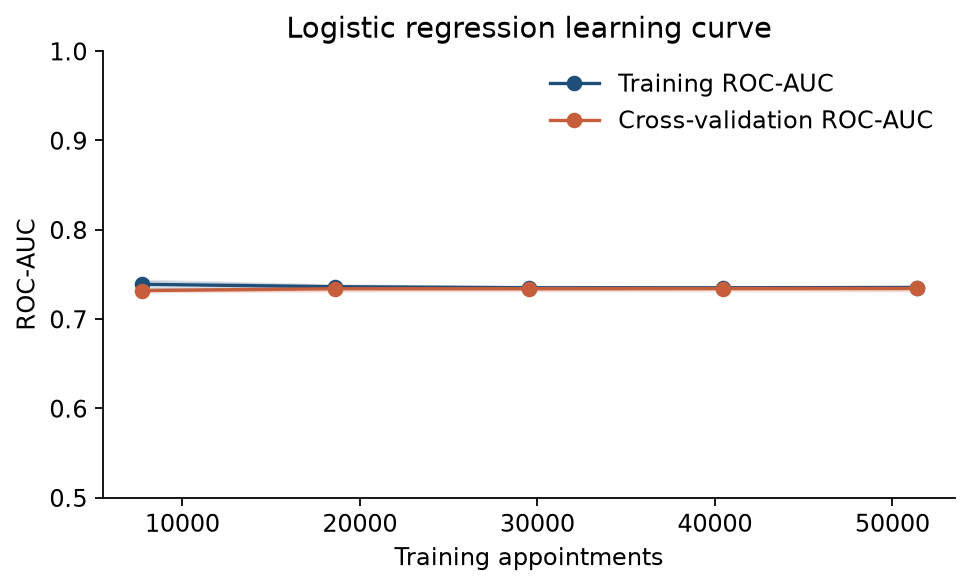
\includegraphics[width=\columnwidth]{../artifacts/figures/learning_curve_logreg.png}
\caption{Logistic regression learning curve on training patients, three-fold ROC-AUC. The curves sit together. Variance is not the problem; the hypothesis class is.}
\label{fig:lc-lr}
\end{figure}

The forests make the variance visible. E6's train--validation gap is 0.019 and its test ROC-AUC is 0.743. E7 reaches a training ROC-AUC of 0.999 against a validation value of 0.749 (gap 0.250), then falls to 0.737 on the test patients, worse than the shallow forest. E8's extra depth buys a test gain of 0.003 over E6 and a gap of 0.131. Fig.~\ref{fig:lc-rf} shows the constrained forest: training ROC-AUC settles from about 0.80 toward 0.77, and cross-validation stays near 0.74--0.75. More rows from this window do not lift the ceiling.

\begin{figure}[t]
\centering
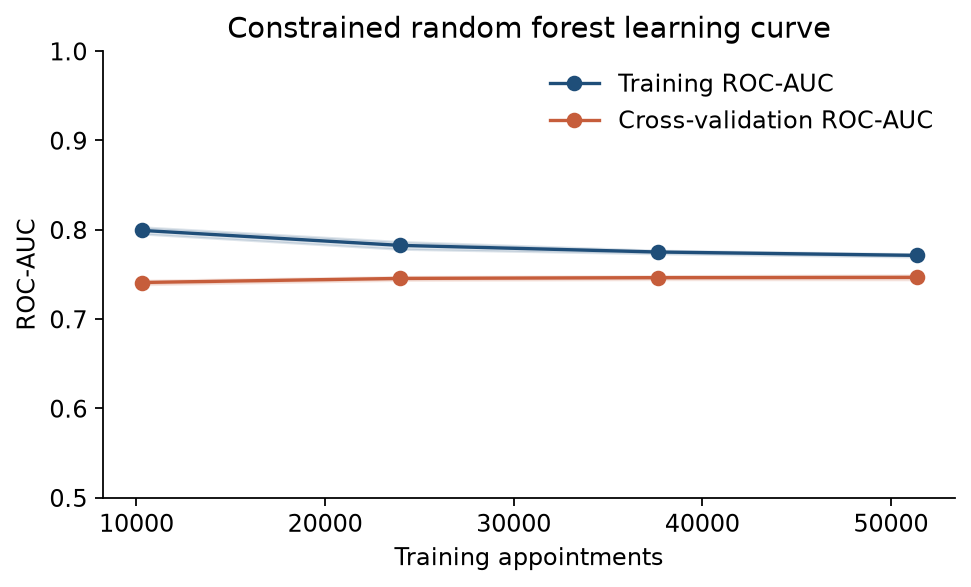
\includegraphics[width=\columnwidth]{../artifacts/figures/learning_curve_forest.png}
\caption{Constrained random forest (depth 8, 80 trees in the curve). Cross-validation is flat. Depth, not sample size, is what E7 spent and did not get back on the test patients.}
\label{fig:lc-rf}
\end{figure}

E9 and E10 have the best validation ROC-AUCs (0.757 and 0.758) and the same test ROC-AUC, 0.748. Shrinkage did the work of E6's depth cap, with a small extra gain \cite{friedman2001}. I keep E10 because the validation rule said so and because its probabilities mean something. E10's test Brier score is 0.140, better than the prevalence constant (about 0.161). E9's is 0.205. Fig.~\ref{fig:cal} shows E10 on the diagonal and the class-weighted models below it: a score near 0.65 from E5 or E15 is an observed rate near 0.30. Once each model has its own F1 threshold, E9 and E10 tie (test F1 0.452 and 0.454). The weights moved the cutoff from 0.55 to 0.225 more than they moved the ranking.

\begin{figure}[t]
\centering
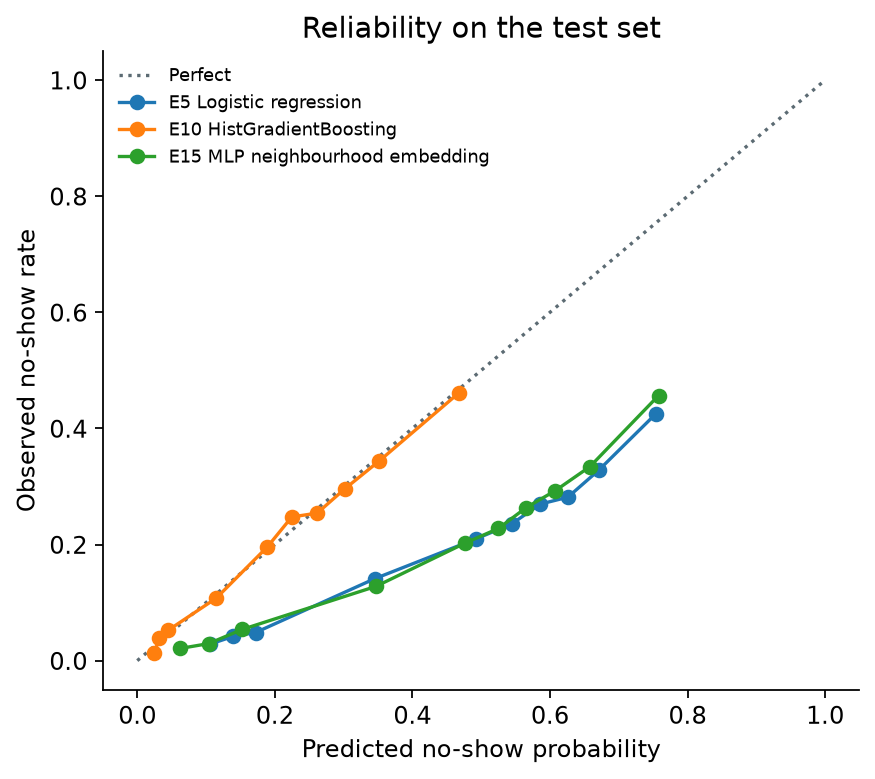
\includegraphics[width=\columnwidth]{../artifacts/figures/calibration_test.png}
\caption{Test-set reliability. The unweighted booster tracks the diagonal. Class-weighted logistic regression and the class-weighted embedding network are systematically too sure.}
\label{fig:cal}
\end{figure}

E11, the linear SVM, matches logistic regression: test ROC-AUC 0.726, and the $C$ grid was flat at 0.734 on validation. The linear separator and the logistic loss are not the difference that matters. E12, the kernel SVM on 8{,}000 rows, is worse on the full validation and test sets (test ROC-AUC 0.712) and has a gap of 0.119 against the subsample it actually fit. Discarding most of the training patients cost more than the nonlinear boundary returned \cite{cortes1995}.

\subsection{Neural nets}
Fig.~\ref{fig:dl} is the epoch curve. E13 stops at epoch 13 with training and validation loss together and a ROC-AUC gap of 0.015. It is not memorising; it is stuck at a test ROC-AUC of 0.737, below the booster. E14 and E15 run to the 25-epoch cap. Their losses sit higher because class weights change the objective, and validation loss does not diverge, so the lower learning rate in E14 was a precaution rather than a rescue from instability \cite{kingma2015}. Validation ROC-AUC flattens below 0.75 for all three nets. E15 is the best of them (test ROC-AUC 0.743) and still short of E10. An embedding that had to learn neighbourhood without the hand-built rate did not beat a booster that was given that rate \cite{goodfellow2016}.

\begin{figure*}[t]
\centering
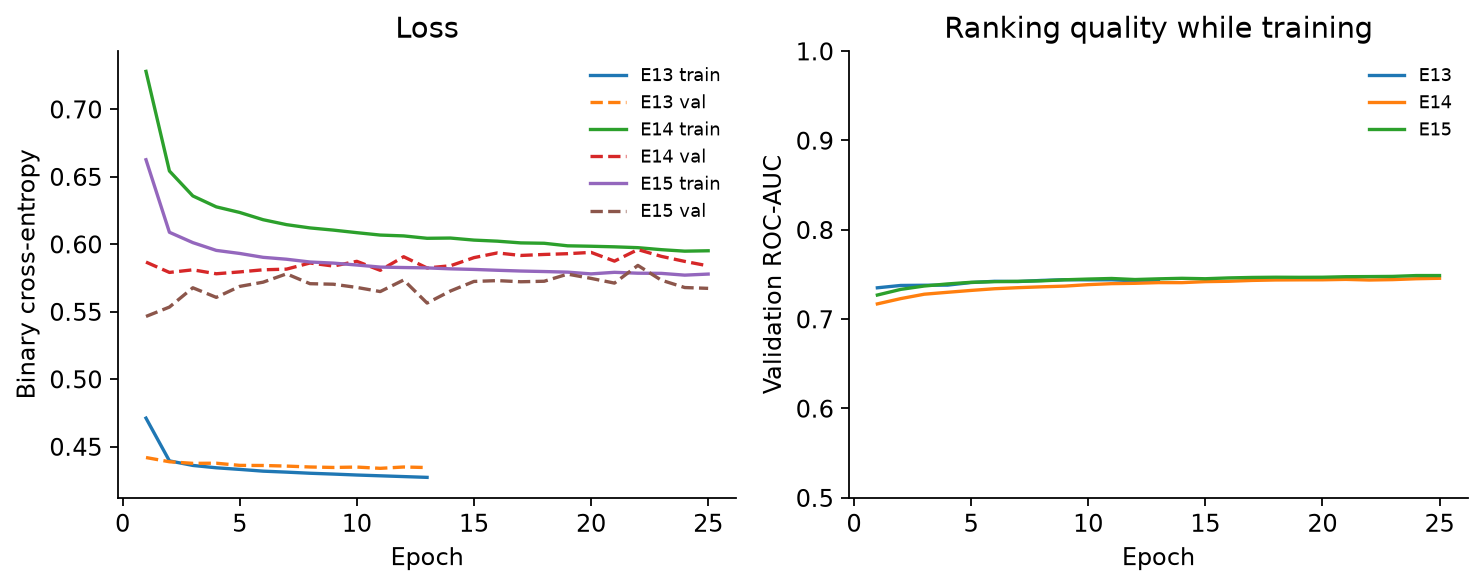
\includegraphics[width=0.92\textwidth]{../artifacts/figures/dl_learning_curves.png}
\caption{Epoch curves for the three networks. E13 stops early with train and validation loss together. E14 and E15, trained with class weights, have a higher loss scale and a flat validation ROC-AUC. None of them pulls away after the first few epochs.}
\label{fig:dl}
\end{figure*}

Fig.~\ref{fig:roc} and Fig.~\ref{fig:pr} overlay the test curves for the lead-time rule, the tuned logistic model, the intermediate forest, the selected booster, the linear SVM, and E15. The ROC plot is flattering: several systems look similarly above the diagonal. The precision--recall plot separates them more honestly and keeps every curve far below the top-right corner \cite{saito2015}. At the recall a clinic would actually want, precision remains well under one half.

\begin{figure}[t]
\centering
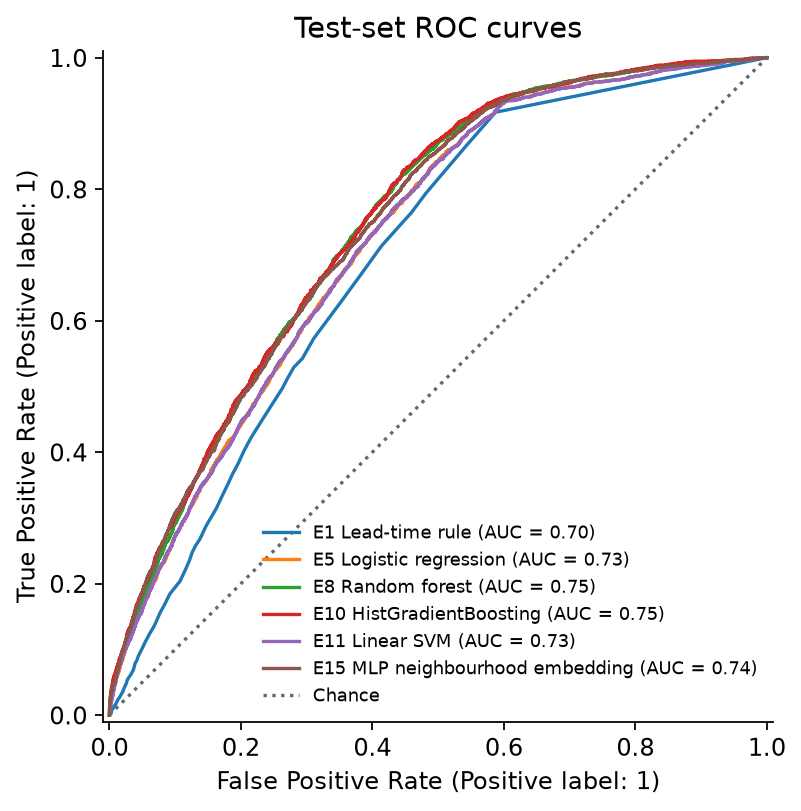
\includegraphics[width=\columnwidth]{../artifacts/figures/roc_test.png}
\caption{Test ROC curves. The lead-time rule carries much of the ranking. Boosting and the embedding network pull ahead by a modest margin.}
\label{fig:roc}
\end{figure}

\begin{figure}[t]
\centering
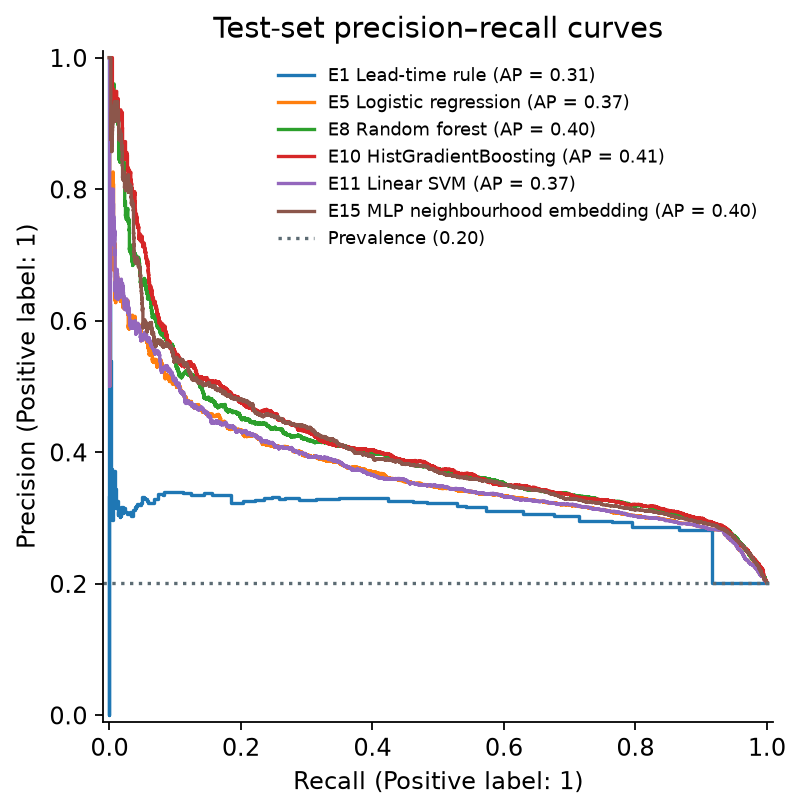
\includegraphics[width=\columnwidth]{../artifacts/figures/pr_test.png}
\caption{Test precision--recall curves. The horizontal reference is the 20\% prevalence. Average precision, not accuracy, is where the models differ in a way a reminder budget would notice.}
\label{fig:pr}
\end{figure}

\subsection{What the selected model uses, and whom it misses}
Permutation importance on E10 (Fig.~\ref{fig:perm}) is dominated by lead time. Shuffling that column drops validation ROC-AUC by about 0.20, which is most of the model's lift over chance. Age is next, then the prior no-show rate, then days since the previous visit. SMS, scholarship, sex, and weekday are close to zero once lead time is present. That is consistent with the adjusted logistic picture and with the stratified SMS rates. The standardised logistic coefficients in Fig.~\ref{fig:coef} need a more cautious reading. Same-day booking has a large negative coefficient ($-0.78$), and log lead time a large positive one ($+0.44$), while raw lead time is slightly negative ($-0.10$). Those three terms are one mechanism split across collinear columns. I do not interpret the negative raw-day coefficient as ``waiting longer reduces no-shows.'' The permutation result forbids that reading. Prior no-show rate ($+0.23$) and age ($-0.21$) are cleaner: a worse personal history raises the log-odds, and older patients have lower log-odds, holding the other standardised columns fixed. The SMS coefficient is negative ($-0.10$) after lead time is in the model, which matches Fig.~\ref{fig:sms} and contradicts the crude association.

\begin{figure}[t]
\centering
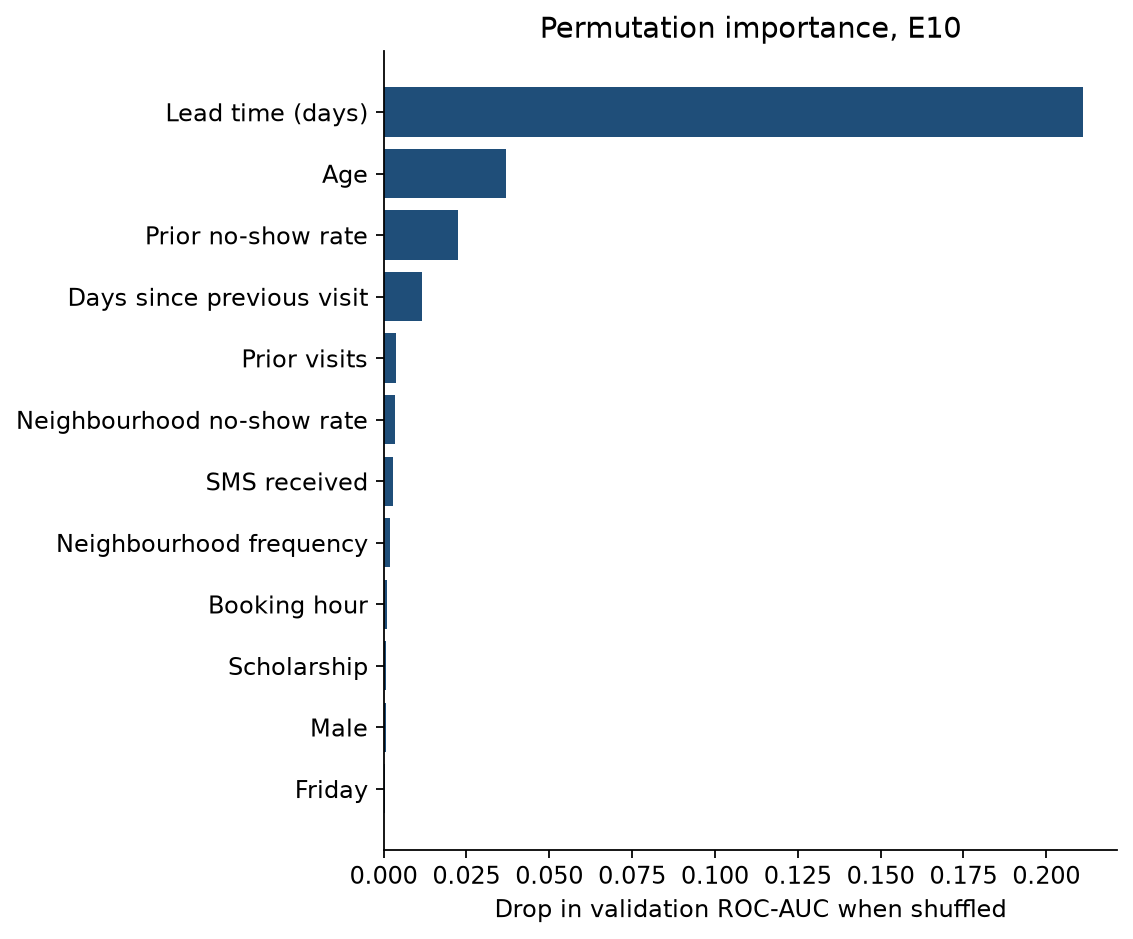
\includegraphics[width=\columnwidth]{../artifacts/figures/permutation_importance.png}
\caption{Permutation importance for E10 on a validation subsample. Lead time is the feature the booster cannot replace. SMS is not, once lead time is known.}
\label{fig:perm}
\end{figure}

\begin{figure}[t]
\centering
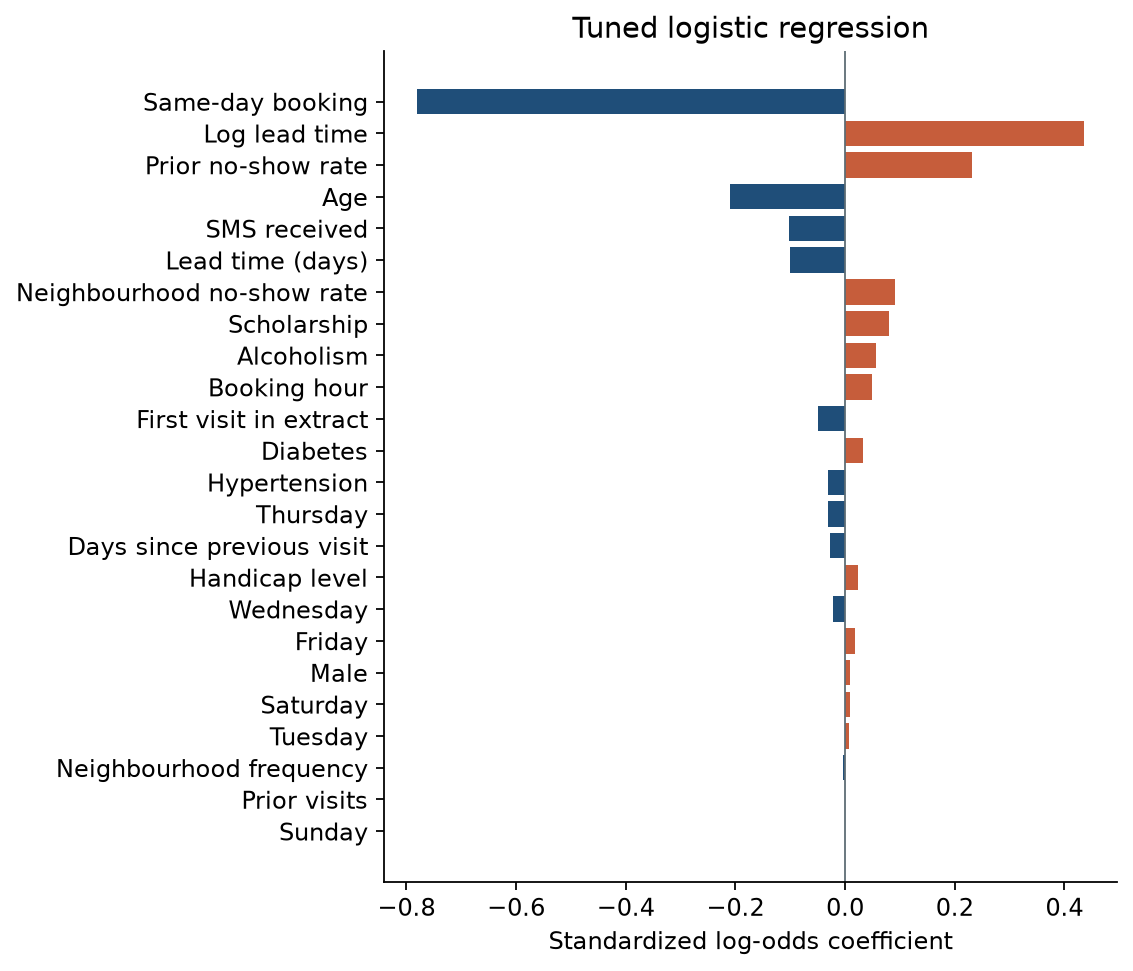
\includegraphics[width=\columnwidth]{../artifacts/figures/logreg_coefficients.png}
\caption{Standardised coefficients from E5. Lead time is spread across three collinear terms. Prior no-show rate and age are the other coefficients large enough to discuss.}
\label{fig:coef}
\end{figure}

At the validation F1 threshold of 0.225, E10's test confusion matrix (Fig.~\ref{fig:cm-ml}) is 8{,}340 true attenders left alone, 5{,}024 attenders flagged, 896 missed no-shows, and 2{,}466 no-shows caught. Precision is 0.329 and recall is 0.733. The model flags 7{,}490 of 16{,}726 test visits, about 45\%. E15's matrix (Fig.~\ref{fig:cm-dl}), at its own threshold of 0.525, is 8{,}264, 5{,}100, 914, and 2{,}448. The network's higher threshold is an artifact of class weights pushing scores up, visible in Fig.~\ref{fig:cal}. The counts of people caught and people bothered are almost the same. Changing the architecture did not change the error budget.

\begin{figure}[t]
\centering
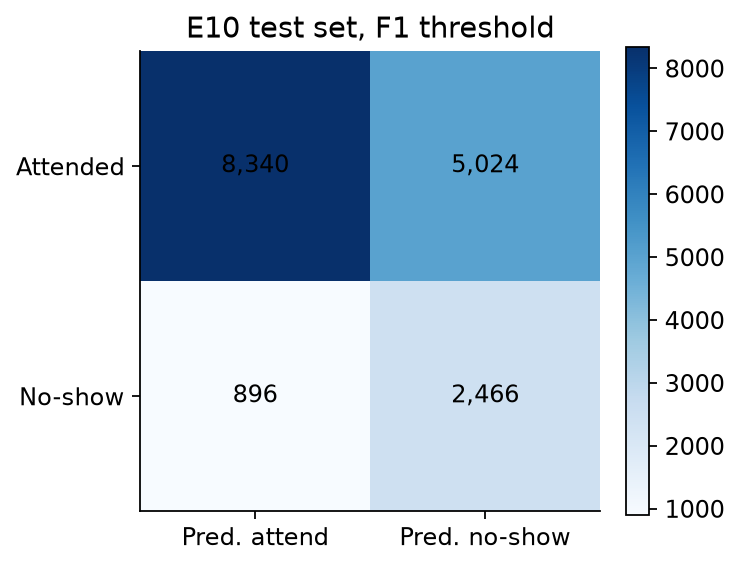
\includegraphics[width=\columnwidth]{../artifacts/figures/confusion_best_traditional.png}
\caption{E10 on the test patients at the F1 threshold locked on validation (0.225). Most detected no-shows are paid for with a large false-positive count.}
\label{fig:cm-ml}
\end{figure}

\begin{figure}[t]
\centering
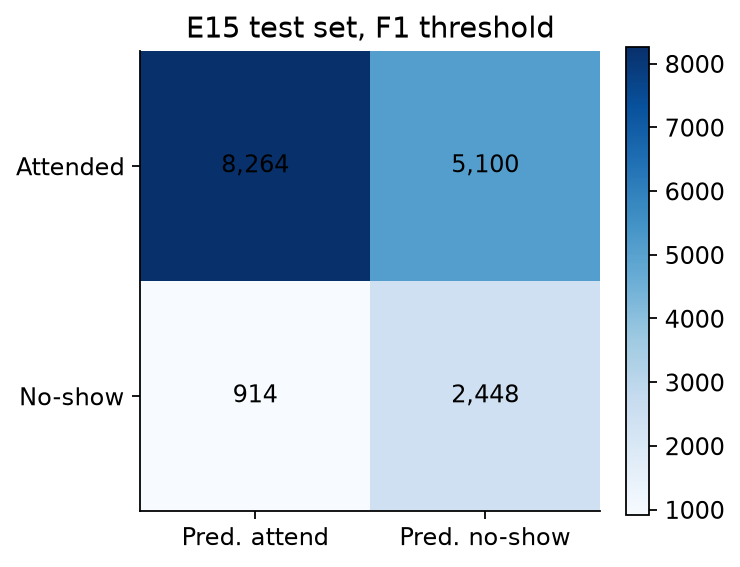
\includegraphics[width=\columnwidth]{../artifacts/figures/confusion_best_deep.png}
\caption{E15 on the same test patients at its own F1 threshold (0.525). The off-diagonal counts are close to Fig.~\ref{fig:cm-ml}.}
\label{fig:cm-dl}
\end{figure}

Table~\ref{tab:policy} applies the four validation-locked policies to E10's test probabilities. The F1 point and the reminder-cost point (threshold 0.25) are neighbours: precision about 0.33--0.34 and recall about 0.65--0.73. They are reasonable if the action is a message. They are not reasonable if the action is a second booking. The overbooking scenario, with a false positive five times as costly as a false negative, moves the threshold to 0.775. Precision rises to 0.908 and recall falls to 0.018. The model does contain a thin tail that is usually right, and that tail covers almost none of the missed visits. Fig.~\ref{fig:trade} shows why. Precision climbs only after the threshold has already given up most of the recall. The capacity rule, flagging the top 20\% of scores, has test precision 0.399 and recall 0.412. Contacting one visit in five catches about two fifths of the no-shows, roughly twice a random list of the same length. That is the most practical summary I can defend.

\begin{table}[t]
\caption{E10 policies on the test set. Thresholds were chosen on validation. Costs are relative units per 1{,}000 visits, not currency.}
\label{tab:policy}
\centering
\footnotesize
\begin{tabular}{lrrrr}
\toprule
Policy & Thr. & Prec. & Recall & Overbook cost \\
\midrule
F1 & 0.225 & 0.329 & 0.733 & 1555 \\
Reminder (FP1, FN3) & 0.250 & 0.344 & 0.653 & 1322 \\
Top 20\% of scores & 0.321 & 0.399 & 0.412 & 742 \\
Cutoff 0.50 & 0.500 & 0.635 & 0.066 & 226 \\
Overbook (FP5, FN1) & 0.775 & 0.908 & 0.018 & 199 \\
\bottomrule
\end{tabular}
\end{table}

\begin{figure}[t]
\centering
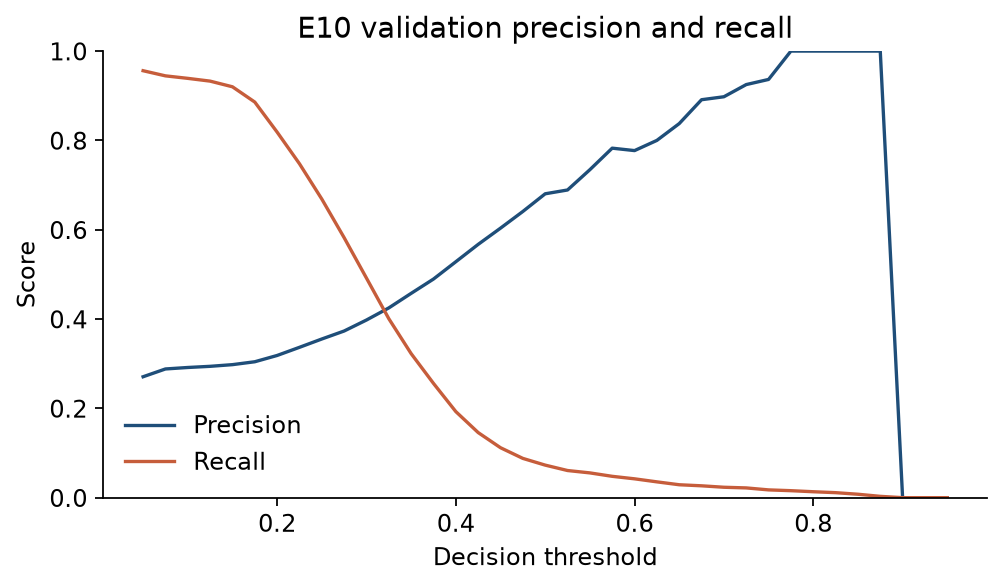
\includegraphics[width=\columnwidth]{../artifacts/figures/threshold_tradeoff_val.png}
\caption{Validation precision and recall for E10 against the decision threshold. The curves cross at a low threshold, which is why an F1 rule flags a large share of the book.}
\label{fig:trade}
\end{figure}

Fig.~\ref{fig:slice} is the error pattern average AUC hides. Same-day test visits have a 4.8\% no-show rate and recall of only 0.16, even though ROC-AUC inside that slice is still 0.71. A global F1 threshold will not spend flags on a 5\% base rate. Recall rises to 0.62 within a week and about 0.88 after that, with precision stuck near 0.34--0.37. Much of the model is the rule ``this visit is not soon.'' Recall is 0.89 at ages 18--39 and 0.36 at 60 and above, against base rates of 23.8\% and 16.0\%. Women and men are close. Scholarship visits are flagged more often, but that flag has almost no permutation importance, so the extra recalls likely travel with lead time. First visits, which have no personal history, have ROC-AUC 0.739 against 0.760 for return visits. History helps a little, which matters for a new digital book full of first visits.

\begin{figure}[t]
\centering
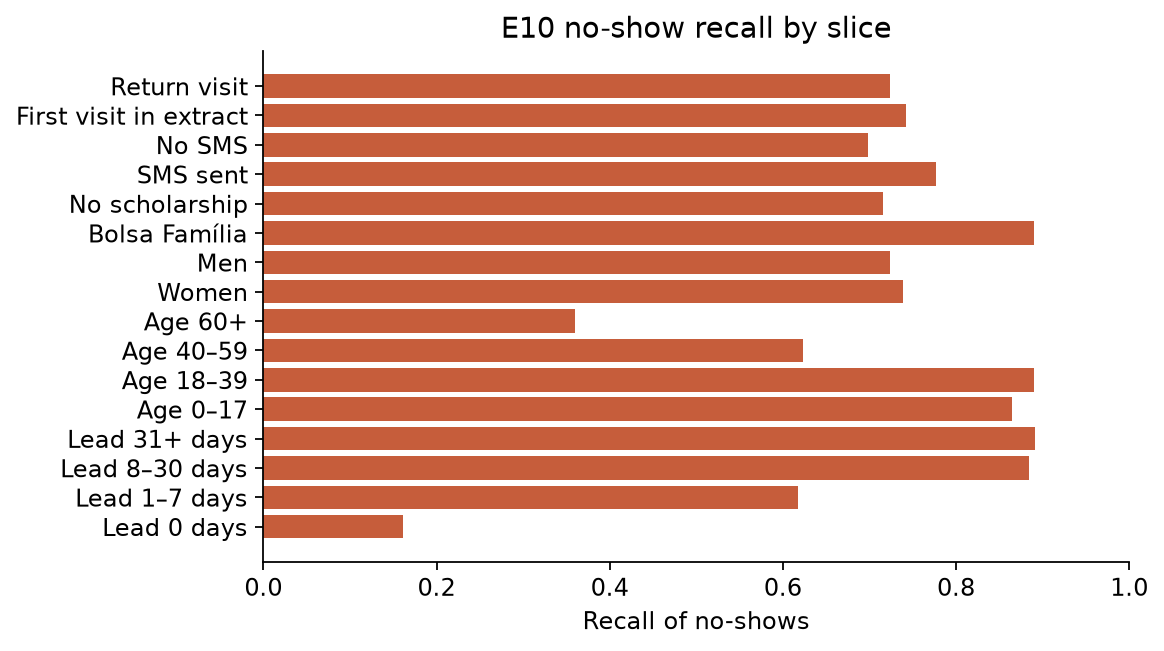
\includegraphics[width=\columnwidth]{../artifacts/figures/slice_recall_test.png}
\caption{E10 recall of test no-shows by slice, at the global F1 threshold. Older patients and same-day visits are systematically under-flagged.}
\label{fig:slice}
\end{figure}

\section{Discussion}
The bias--variance reading is direct \cite{geman1992}. The logistic learning curve is two overlapping flat lines, which is high bias and low variance. E7 is the opposite: training ROC-AUC of 0.999, a validation gap of 0.250, and a test score worse than a forest that was forbidden from making pure leaves. E10 keeps a gap of 0.017 and the best test ranking. That is the usual argument for shrinkage and early stopping, observed here rather than cited as a slogan \cite{friedman2001}. The neural curves add a third pattern. They do not overfit in the dramatic sense, and they also do not reach the booster. The residual is not a shortage of epochs or an unstable step size. It is a label that is mostly a step function of lead time, which a tree splits in one cut and which a smooth network spends capacity approximating. I would not move to a deeper net, or to a transformer over visits, until the table contains a reason for the visit, a distance, or a record of why the last appointment was missed. Those fields are how Mohammadi \emph{et al.} got a richer model \cite{mohammadi2018}. Architecture will not invent them.

The operational reading is less comfortable than the AUC. At the F1 point the model is wrong about two thirds of the people it flags. That can still be a reasonable SMS policy where a message changed attendance \cite{thomas2017} and a reminder to everyone did not \cite{kheirkhah2016}. It is a bad overbooking policy in a room that already waits for hours \cite{oche2013}. Under a 5:1 false-positive penalty the safe tail covers under 2\% of no-shows, so this file does not reproduce the aggressive double-booking Huang and Hanauer could justify in their clinic \cite{huang2014}. The product I would pilot is the top fifth of the score, not an automatic second appointment.

There is a larger intervention sitting in Fig.~\ref{fig:lead}. Same-day visits miss at 4.5\%. Visits booked two weeks ahead miss at about 31\%. A booking policy that offers more near-term slots changes the base rate by an amount no classifier in this study matched. Levesque's access framework is the right language for that result \cite{levesque2013}. Lead time is not a patient trait. It is a slot the clinic did or did not have. Prediction is what you do for the visits that must be booked ahead. It is a poor substitute for capacity.

The same global threshold is not equity-neutral \cite{rajkomar2018}. Older no-shows are recalled at 0.36 and younger adults at 0.89. A clinic that spent reminder effort in score order would favour the patients the model finds easy. Group-specific thresholds were not fit. Neighbourhood target encoding can also carry social geography into a number staff will treat as clinical.

What this study cannot support is a claim about African clinics. The window is six weeks in one Brazilian city, with no distance, diagnosis, or reason a visit was missed. Bolsa Familia does not transfer as a socioeconomic measure. Dantas \emph{et al.} put African no-show rates near 43\%, so every probability here would need to be re-fit \cite{dantas2018}. Holst \emph{et al.} and the WHO strategy both treat an imported model as something other than a health-system intervention \cite{holst2020,who2021}. The transportable piece is the design: log booking time and outcome, do not leak history across patients, and judge reminders and overbooking at different thresholds. A prospective check---freeze the score and compare reminder cost and waiting-room load with usual practice---is the measurement that would replace this offline AUC \cite{huang2014,thomas2017}. Until then the AUC is an upper bound computed in the wrong health system.

\section{Conclusion}
Missed visits in this table are predictable enough to rank and not predictable enough to double-book. Sixteen patient-grouped experiments put an unweighted gradient booster first (test ROC-AUC 0.748, average precision 0.411). A neighbourhood-embedding network is close and does not justify the extra machinery. Lead time, then age and prior non-attendance, carry the ranking. An unrestricted forest memorises, and class weights distort probabilities once the threshold is free to move. The F1 point catches about three quarters of no-shows and is wrong on about two thirds of its flags; a high-precision point covers under 2\% of no-shows. The use that fits the evidence is a limited reminder list. A same-day slot changes attendance more than the model does. None of these thresholds belongs in an African clinic that has not trained on its own outcomes.

\begin{thebibliography}{99}
\bibitem{oche2013} M.~O. Oche and H.~Adamu, ``Determinants of patient waiting time in the general outpatient department of a tertiary health institution in North Western Nigeria,'' \emph{Ann. Med. Health Sci. Res.}, vol.~3, no.~4, pp.~588--592, 2013, doi: 10.4103/2141-9248.122123.
\bibitem{dantas2018} L.~F. Dantas, J.~L. Fleck, F.~L. Cyrino Oliveira, and S.~Hamacher, ``No-shows in appointment scheduling -- a systematic literature review,'' \emph{Health Policy}, vol.~122, no.~4, pp.~412--421, Apr. 2018, doi: 10.1016/j.healthpol.2018.02.002.
\bibitem{carreras2020} D.~Carreras-Garc\'ia, D.~Delgado-G\'omez, F.~Llorente-Fern\'andez, and A.~Arribas-Gil, ``Patient no-show prediction: A systematic literature review,'' \emph{Entropy}, vol.~22, no.~6, p.~675, Jun. 2020, doi: 10.3390/e22060675.
\bibitem{huang2014} Y.~Huang and D.~A. Hanauer, ``Patient no-show predictive model development using multiple data sources for an effective overbooking approach,'' \emph{Appl. Clin. Inform.}, vol.~5, no.~3, pp.~836--860, 2014, doi: 10.4338/ACI-2014-04-RA-0026.
\bibitem{hoppen2016} J.~Hoppen, ``Medical appointment no shows,'' Kaggle dataset, May 2016. [Online]. Available: \url{https://www.kaggle.com/datasets/joniarroba/noshowappointments}
\bibitem{mohammadi2018} I.~Mohammadi, H.~Wu, A.~Turkcan, T.~Toscos, and B.~N. Doebbeling, ``Data analytics and modeling for appointment no-show in community health centers,'' \emph{J. Primary Care Community Health}, vol.~9, 2018, doi: 10.1177/2150132718811692.
\bibitem{kheirkhah2016} P.~Kheirkhah, Q.~Feng, L.~M. Travis, S.~Tavakoli-Tabasi, and A.~Sharafkhaneh, ``Prevalence, predictors and economic consequences of no-shows,'' \emph{BMC Health Serv. Res.}, vol.~16, p.~13, Jan. 2016, doi: 10.1186/s12913-015-1243-z.
\bibitem{thomas2017} I.~F. Thomas, A.~O. Lawani, and B.~O. James, ``Effect of short message service reminders on clinic attendance among outpatients with psychosis at a psychiatric hospital in Nigeria,'' \emph{Psychiatr. Serv.}, vol.~68, no.~1, Jan. 2017, doi: 10.1176/appi.ps.201500514.
\bibitem{akhigbe2014} S.~Akhigbe, O.~Morakinyo, A.~Lawani, \emph{et al.}, ``Prevalence and correlates of missed first appointments among outpatients at a psychiatric hospital in Nigeria,'' \emph{Ann. Med. Health Sci. Res.}, vol.~4, pp.~763--768, 2014.
\bibitem{gurol2013} I.~Gurol-Urganci, T.~de~Jongh, V.~Vodopivec-Jamsek, R.~Atun, and J.~Car, ``Mobile phone messaging reminders for attendance at healthcare appointments,'' \emph{Cochrane Database Syst. Rev.}, no.~12, Art.~no.~CD007458, 2013, doi: 10.1002/14651858.CD007458.pub3.
\bibitem{levesque2013} J.-F. Levesque, M.~F. Harris, and G.~Russell, ``Patient-centred access to health care: Conceptualising access at the interface of health systems and populations,'' \emph{Int. J. Equity Health}, vol.~12, p.~18, 2013, doi: 10.1186/1475-9276-12-18.
\bibitem{holst2020} C.~Holst, F.~Sukums, D.~Radovanovi\'c, B.~Ngowi, J.~Noll, and A.~S. Winkler, ``Sub-Saharan Africa---the new breeding ground for global digital health,'' \emph{Lancet Digit. Health}, vol.~2, no.~4, Apr. 2020, doi: 10.1016/S2589-7500(20)30027-3.
\bibitem{who2021} World Health Organization, \emph{Global Strategy on Digital Health 2020--2025}. Geneva, Switzerland: WHO, 2021.
\bibitem{hastie2009} T.~Hastie, R.~Tibshirani, and J.~Friedman, \emph{The Elements of Statistical Learning}, 2nd~ed. New York, NY, USA: Springer, 2009.
\bibitem{geman1992} S.~Geman, E.~Bienenstock, and R.~Doursat, ``Neural networks and the bias/variance dilemma,'' \emph{Neural Comput.}, vol.~4, no.~1, pp.~1--58, 1992.
\bibitem{breiman2001} L.~Breiman, ``Random forests,'' \emph{Mach. Learn.}, vol.~45, no.~1, pp.~5--32, 2001.
\bibitem{friedman2001} J.~H. Friedman, ``Greedy function approximation: A gradient boosting machine,'' \emph{Ann. Statist.}, vol.~29, no.~5, pp.~1189--1232, 2001.
\bibitem{cortes1995} C.~Cortes and V.~Vapnik, ``Support-vector networks,'' \emph{Mach. Learn.}, vol.~20, no.~3, pp.~273--297, 1995.
\bibitem{goodfellow2016} I.~Goodfellow, Y.~Bengio, and A.~Courville, \emph{Deep Learning}. Cambridge, MA, USA: MIT Press, 2016.
\bibitem{srivastava2014} N.~Srivastava, G.~Hinton, A.~Krizhevsky, I.~Sutskever, and R.~Salakhutdinov, ``Dropout: A simple way to prevent neural networks from overfitting,'' \emph{J. Mach. Learn. Res.}, vol.~15, pp.~1929--1958, 2014.
\bibitem{ioffe2015} S.~Ioffe and C.~Szegedy, ``Batch normalization: Accelerating deep network training by reducing internal covariate shift,'' in \emph{Proc. 32nd Int. Conf. Mach. Learn.}, 2015, pp.~448--456.
\bibitem{kingma2015} D.~P. Kingma and J.~Ba, ``Adam: A method for stochastic optimization,'' in \emph{Proc. Int. Conf. Learn. Represent.}, 2015.
\bibitem{saito2015} T.~Saito and M.~Rehmsmeier, ``The precision-recall plot is more informative than the ROC plot when evaluating binary classifiers on imbalanced datasets,'' \emph{PLoS ONE}, vol.~10, no.~3, Art.~no.~e0118432, Mar. 2015, doi: 10.1371/journal.pone.0118432.
\bibitem{chawla2002} N.~V. Chawla, K.~W. Bowyer, L.~O. Hall, and W.~P. Kegelmeyer, ``SMOTE: Synthetic minority over-sampling technique,'' \emph{J. Artif. Intell. Res.}, vol.~16, pp.~321--357, 2002.
\bibitem{kaufman2012} S.~Kaufman, S.~Rosset, C.~Perlich, and O.~Stitelman, ``Leakage in data mining: Formulation, detection, and avoidance,'' \emph{ACM Trans. Knowl. Discov. Data}, vol.~6, no.~4, Art.~no.~15, Dec. 2012, doi: 10.1145/2382577.2382578.
\bibitem{rajkomar2018} A.~Rajkomar, M.~Hardt, M.~D. Howell, G.~Corrado, and M.~H. Chin, ``Ensuring fairness in machine learning to advance health equity,'' \emph{Ann. Intern. Med.}, vol.~169, no.~12, pp.~866--872, Dec. 2018, doi: 10.7326/M18-1990.
\end{thebibliography}

\end{document}
